\documentclass[twoside]{book}

% Packages required by doxygen
\usepackage{fixltx2e}
\usepackage{calc}
\usepackage{doxygen}
\usepackage[export]{adjustbox} % also loads graphicx
\usepackage{graphicx}
\usepackage[utf8]{inputenc}
\usepackage{makeidx}
\usepackage{multicol}
\usepackage{multirow}
\PassOptionsToPackage{warn}{textcomp}
\usepackage{textcomp}
\usepackage[nointegrals]{wasysym}
\usepackage[table]{xcolor}

% Font selection
\usepackage[T1]{fontenc}
\usepackage[scaled=.90]{helvet}
\usepackage{courier}
\usepackage{amssymb}
\usepackage{sectsty}
\renewcommand{\familydefault}{\sfdefault}
\allsectionsfont{%
  \fontseries{bc}\selectfont%
  \color{darkgray}%
}
\renewcommand{\DoxyLabelFont}{%
  \fontseries{bc}\selectfont%
  \color{darkgray}%
}
\newcommand{\+}{\discretionary{\mbox{\scriptsize$\hookleftarrow$}}{}{}}

% Page & text layout
\usepackage{geometry}
\geometry{%
  a4paper,%
  top=2.5cm,%
  bottom=2.5cm,%
  left=2.5cm,%
  right=2.5cm%
}
\tolerance=750
\hfuzz=15pt
\hbadness=750
\setlength{\emergencystretch}{15pt}
\setlength{\parindent}{0cm}
\setlength{\parskip}{3ex plus 2ex minus 2ex}
\makeatletter
\renewcommand{\paragraph}{%
  \@startsection{paragraph}{4}{0ex}{-1.0ex}{1.0ex}{%
    \normalfont\normalsize\bfseries\SS@parafont%
  }%
}
\renewcommand{\subparagraph}{%
  \@startsection{subparagraph}{5}{0ex}{-1.0ex}{1.0ex}{%
    \normalfont\normalsize\bfseries\SS@subparafont%
  }%
}
\makeatother

% Headers & footers
\usepackage{fancyhdr}
\pagestyle{fancyplain}
\fancyhead[LE]{\fancyplain{}{\bfseries\thepage}}
\fancyhead[CE]{\fancyplain{}{}}
\fancyhead[RE]{\fancyplain{}{\bfseries\leftmark}}
\fancyhead[LO]{\fancyplain{}{\bfseries\rightmark}}
\fancyhead[CO]{\fancyplain{}{}}
\fancyhead[RO]{\fancyplain{}{\bfseries\thepage}}
\fancyfoot[LE]{\fancyplain{}{}}
\fancyfoot[CE]{\fancyplain{}{}}
\fancyfoot[RE]{\fancyplain{}{\bfseries\scriptsize Generated by Doxygen }}
\fancyfoot[LO]{\fancyplain{}{\bfseries\scriptsize Generated by Doxygen }}
\fancyfoot[CO]{\fancyplain{}{}}
\fancyfoot[RO]{\fancyplain{}{}}
\renewcommand{\footrulewidth}{0.4pt}
\renewcommand{\chaptermark}[1]{%
  \markboth{#1}{}%
}
\renewcommand{\sectionmark}[1]{%
  \markright{\thesection\ #1}%
}

% Indices & bibliography
\usepackage{natbib}
\usepackage[titles]{tocloft}
\setcounter{tocdepth}{3}
\setcounter{secnumdepth}{5}
\makeindex

% Hyperlinks (required, but should be loaded last)
\usepackage{ifpdf}
\ifpdf
  \usepackage[pdftex,pagebackref=true]{hyperref}
\else
  \usepackage[ps2pdf,pagebackref=true]{hyperref}
\fi
\hypersetup{%
  colorlinks=true,%
  linkcolor=blue,%
  citecolor=blue,%
  unicode%
}

% Custom commands
\newcommand{\clearemptydoublepage}{%
  \newpage{\pagestyle{empty}\cleardoublepage}%
}

\usepackage{caption}
\captionsetup{labelsep=space,justification=centering,font={bf},singlelinecheck=off,skip=4pt,position=top}

%===== C O N T E N T S =====

\begin{document}

% Titlepage & ToC
\hypersetup{pageanchor=false,
             bookmarksnumbered=true,
             pdfencoding=unicode
            }
\pagenumbering{alph}
\begin{titlepage}
\vspace*{7cm}
\begin{center}%
{\Large My Project }\\
\vspace*{1cm}
{\large Generated by Doxygen 1.8.13}\\
\end{center}
\end{titlepage}
\clearemptydoublepage
\pagenumbering{roman}
\tableofcontents
\clearemptydoublepage
\pagenumbering{arabic}
\hypersetup{pageanchor=true}

%--- Begin generated contents ---
\chapter{Deprecated List}
\label{deprecated}
\Hypertarget{deprecated}

\begin{DoxyRefList}
\item[\label{deprecated__deprecated000001}%
\Hypertarget{deprecated__deprecated000001}%
Member \hyperlink{coindex-getopt_8h_a78a0cd581698415a62f68214603b1a30}{cmdline\+\_\+parser2} (int argc, char $\ast$$\ast$argv, struct \hyperlink{structgengetopt__args__info}{gengetopt\+\_\+args\+\_\+info} $\ast$args\+\_\+info, int override, int initialize, int check\+\_\+required)]use \hyperlink{coindex-getopt_8h_ac7bb5d76f3f56d1c0b3b531f11ac6f07}{cmdline\+\_\+parser\+\_\+ext()} instead 

use \hyperlink{coindex-getopt_8h_ac7bb5d76f3f56d1c0b3b531f11ac6f07}{cmdline\+\_\+parser\+\_\+ext()} instead 

use \hyperlink{coindex-getopt_8h_ac7bb5d76f3f56d1c0b3b531f11ac6f07}{cmdline\+\_\+parser\+\_\+ext()} instead 

use \hyperlink{coindex-getopt_8h_ac7bb5d76f3f56d1c0b3b531f11ac6f07}{cmdline\+\_\+parser\+\_\+ext()} instead 
\end{DoxyRefList}
\chapter{Hierarchical Index}
\section{Class Hierarchy}
This inheritance list is sorted roughly, but not completely, alphabetically\+:\begin{DoxyCompactList}
\item \contentsline{section}{A}{\pageref{classA}}{}
\item \contentsline{section}{Classic\+Cipher}{\pageref{classClassicCipher}}{}
\begin{DoxyCompactList}
\item \contentsline{section}{Vigenere\+Cipher}{\pageref{classVigenereCipher}}{}
\begin{DoxyCompactList}
\item \contentsline{section}{Vigenere\+Breaker}{\pageref{classVigenereBreaker}}{}
\end{DoxyCompactList}
\end{DoxyCompactList}
\item \contentsline{section}{cmdline\+\_\+parser\+\_\+params}{\pageref{structcmdline__parser__params}}{}
\item \contentsline{section}{custom\+\_\+getopt\+\_\+data}{\pageref{structcustom__getopt__data}}{}
\item \contentsline{section}{gengetopt\+\_\+args\+\_\+info}{\pageref{structgengetopt__args__info}}{}
\item \contentsline{section}{option}{\pageref{structoption}}{}
\item \contentsline{section}{P\+R\+NG}{\pageref{classPRNG}}{}
\begin{DoxyCompactList}
\item \contentsline{section}{Blum\+Blum\+Shub\+Generator}{\pageref{classBlumBlumShubGenerator}}{}
\end{DoxyCompactList}
\end{DoxyCompactList}

\chapter{Class Index}
\section{Class List}
Here are the classes, structs, unions and interfaces with brief descriptions\+:\begin{DoxyCompactList}
\item\contentsline{section}{\hyperlink{classBlumBlumShubGenerator}{Blum\+Blum\+Shub\+Generator} }{\pageref{classBlumBlumShubGenerator}}{}
\item\contentsline{section}{\hyperlink{classPRNG}{P\+R\+NG} }{\pageref{classPRNG}}{}
\end{DoxyCompactList}

\chapter{File Index}
\section{File List}
Here is a list of all documented files with brief descriptions\+:\begin{DoxyCompactList}
\item\contentsline{section}{/home/sinflair/\+P/crypto/\+A\+K/src/\+Praktikum-\/\+D\+E\+S/{\bfseries Block\+Cipher.\+h} }{\pageref{BlockCipher_8h}}{}
\item\contentsline{section}{/home/sinflair/\+P/crypto/\+A\+K/src/\+Praktikum-\/\+D\+E\+S/{\bfseries byte.\+h} }{\pageref{byte_8h}}{}
\item\contentsline{section}{/home/sinflair/\+P/crypto/\+A\+K/src/\+Praktikum-\/\+D\+E\+S/{\bfseries catch.\+hpp} }{\pageref{catch_8hpp}}{}
\item\contentsline{section}{/home/sinflair/\+P/crypto/\+A\+K/src/\+Praktikum-\/\+D\+E\+S/\hyperlink{des-getopt_8h}{des-\/getopt.\+h} \\*The header file for the command line option parser generated by G\+NU Gengetopt version 2.\+22.\+6 \href{http://www.gnu.org/software/gengetopt}{\tt http\+://www.\+gnu.\+org/software/gengetopt}. DO N\+OT modify this file, since it can be overwritten }{\pageref{des-getopt_8h}}{}
\item\contentsline{section}{/home/sinflair/\+P/crypto/\+A\+K/src/\+Praktikum-\/\+D\+E\+S/{\bfseries D\+E\+S\+Cipher.\+h} }{\pageref{DESCipher_8h}}{}
\end{DoxyCompactList}

\chapter{Class Documentation}
\hypertarget{classAESCipher}{}\section{A\+E\+S\+Cipher Class Reference}
\label{classAESCipher}\index{A\+E\+S\+Cipher@{A\+E\+S\+Cipher}}


Inheritance diagram for A\+E\+S\+Cipher\+:
\nopagebreak
\begin{figure}[H]
\begin{center}
\leavevmode
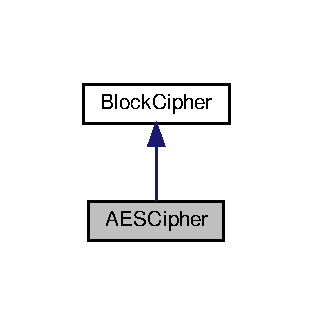
\includegraphics[width=150pt]{classAESCipher__inherit__graph}
\end{center}
\end{figure}


Collaboration diagram for A\+E\+S\+Cipher\+:
\nopagebreak
\begin{figure}[H]
\begin{center}
\leavevmode
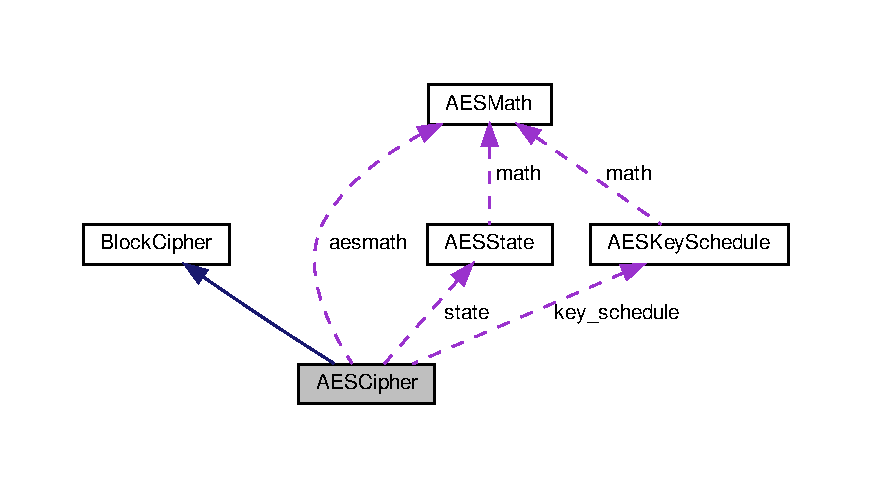
\includegraphics[width=350pt]{classAESCipher__coll__graph}
\end{center}
\end{figure}
\subsection*{Public Member Functions}
\begin{DoxyCompactItemize}
\item 
\mbox{\Hypertarget{classAESCipher_a6356fad966558b8f7219d3a20b9a7656}\label{classAESCipher_a6356fad966558b8f7219d3a20b9a7656}} 
{\bfseries A\+E\+S\+Cipher} (bool debug\+\_\+mode=false)
\item 
\mbox{\Hypertarget{classAESCipher_aa0a48f50b134d4b23b48d147cbb9c395}\label{classAESCipher_aa0a48f50b134d4b23b48d147cbb9c395}} 
bool {\bfseries set\+Key} (const vector$<$ byte $>$ \&key)
\item 
\mbox{\Hypertarget{classAESCipher_af580c4fbade685bca77953f9600c98f3}\label{classAESCipher_af580c4fbade685bca77953f9600c98f3}} 
void {\bfseries encrypt\+Block} (const byte $\ast$plain\+\_\+text, byte $\ast$cipher\+\_\+text)
\item 
\mbox{\Hypertarget{classAESCipher_af0503d3a0ce1090ddb8d0a4ef7ebbe0b}\label{classAESCipher_af0503d3a0ce1090ddb8d0a4ef7ebbe0b}} 
void {\bfseries decrypt\+Block} (const byte $\ast$cipher\+\_\+text, byte $\ast$plain\+\_\+text)
\item 
\mbox{\Hypertarget{classAESCipher_a6bacb932c48a04c050921ce343018eb5}\label{classAESCipher_a6bacb932c48a04c050921ce343018eb5}} 
bool {\bfseries process} (const vector$<$ byte $>$ \&in, vector$<$ byte $>$ \&out, bool mode)
\item 
\mbox{\Hypertarget{classAESCipher_a7bdb3f04dd3c3ee3d286a5c8b3891ea1}\label{classAESCipher_a7bdb3f04dd3c3ee3d286a5c8b3891ea1}} 
bool {\bfseries encrypt} (const vector$<$ byte $>$ \&plain\+\_\+text, vector$<$ byte $>$ \&cipher\+\_\+text)
\item 
\mbox{\Hypertarget{classAESCipher_a51736a7005168423ddee6c07ea3b59a7}\label{classAESCipher_a51736a7005168423ddee6c07ea3b59a7}} 
bool {\bfseries decrypt} (const vector$<$ byte $>$ \&cipher\+\_\+text, vector$<$ byte $>$ \&plain\+\_\+text)
\end{DoxyCompactItemize}
\subsection*{Static Public Member Functions}
\begin{DoxyCompactItemize}
\item 
\mbox{\Hypertarget{classAESCipher_a239e44d62202daa71deb4a212f265033}\label{classAESCipher_a239e44d62202daa71deb4a212f265033}} 
static vector$<$ byte $>$ {\bfseries to\+Vector} (const string \&msg, size\+\_\+t block\+\_\+len=16)
\item 
\mbox{\Hypertarget{classAESCipher_ade366941f98c89b610588ab769ad24fa}\label{classAESCipher_ade366941f98c89b610588ab769ad24fa}} 
static string {\bfseries to\+String} (const vector$<$ byte $>$ \&vec)
\end{DoxyCompactItemize}
\subsection*{Static Public Attributes}
\begin{DoxyCompactItemize}
\item 
\mbox{\Hypertarget{classAESCipher_af100a312dbbee903a9500a87e72895a6}\label{classAESCipher_af100a312dbbee903a9500a87e72895a6}} 
static const bool {\bfseries Encryption} =false
\item 
\mbox{\Hypertarget{classAESCipher_a61687ed03866ee1a8b6dd42a460fec9c}\label{classAESCipher_a61687ed03866ee1a8b6dd42a460fec9c}} 
static const bool {\bfseries Decryption} =true
\end{DoxyCompactItemize}
\subsection*{Private Member Functions}
\begin{DoxyCompactItemize}
\item 
\mbox{\Hypertarget{classAESCipher_ae58dc19b08c7c70a4d078714cecab9b1}\label{classAESCipher_ae58dc19b08c7c70a4d078714cecab9b1}} 
void {\bfseries debug\+Message} (size\+\_\+t round, string msg)
\end{DoxyCompactItemize}
\subsection*{Private Attributes}
\begin{DoxyCompactItemize}
\item 
\mbox{\Hypertarget{classAESCipher_a6809a0219f4fb1b4f36ab094a1da9d89}\label{classAESCipher_a6809a0219f4fb1b4f36ab094a1da9d89}} 
bool {\bfseries debug\+\_\+mode}
\item 
\mbox{\Hypertarget{classAESCipher_a968741a17b9fdc692454b10b39dc104e}\label{classAESCipher_a968741a17b9fdc692454b10b39dc104e}} 
\hyperlink{classAESMath}{A\+E\+S\+Math} {\bfseries aesmath}
\item 
\mbox{\Hypertarget{classAESCipher_afb744a0b2530339e42d3e0c14a75d3a9}\label{classAESCipher_afb744a0b2530339e42d3e0c14a75d3a9}} 
\hyperlink{classAESKeySchedule}{A\+E\+S\+Key\+Schedule} {\bfseries key\+\_\+schedule}
\item 
\mbox{\Hypertarget{classAESCipher_a63a10fb1c42ee469700e57df0618262d}\label{classAESCipher_a63a10fb1c42ee469700e57df0618262d}} 
\hyperlink{classAESState}{A\+E\+S\+State} {\bfseries state}
\end{DoxyCompactItemize}
\subsection*{Additional Inherited Members}


The documentation for this class was generated from the following files\+:\begin{DoxyCompactItemize}
\item 
/home/sinflair/\+P/crypto/\+A\+K/src/\+Praktikum-\/\+A\+E\+S/A\+E\+S\+Cipher.\+h\item 
/home/sinflair/\+P/crypto/\+A\+K/src/\+Praktikum-\/\+A\+E\+S/A\+E\+S\+Cipher.\+cpp\end{DoxyCompactItemize}

\hypertarget{classAESKeySchedule}{}\section{A\+E\+S\+Key\+Schedule Class Reference}
\label{classAESKeySchedule}\index{A\+E\+S\+Key\+Schedule@{A\+E\+S\+Key\+Schedule}}


Collaboration diagram for A\+E\+S\+Key\+Schedule\+:
\nopagebreak
\begin{figure}[H]
\begin{center}
\leavevmode
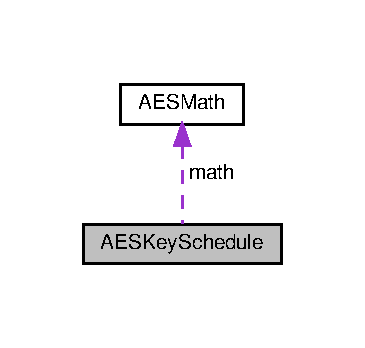
\includegraphics[width=175pt]{classAESKeySchedule__coll__graph}
\end{center}
\end{figure}
\subsection*{Public Member Functions}
\begin{DoxyCompactItemize}
\item 
\mbox{\Hypertarget{classAESKeySchedule_a8f2b4c390d4e2c15d9c40d913ca13569}\label{classAESKeySchedule_a8f2b4c390d4e2c15d9c40d913ca13569}} 
word {\bfseries rot\+Word} (word w) const
\item 
\mbox{\Hypertarget{classAESKeySchedule_a2c36c243dfca9d1e14b2f51a54a7ba08}\label{classAESKeySchedule_a2c36c243dfca9d1e14b2f51a54a7ba08}} 
word {\bfseries sub\+Word} (word w) const
\item 
\mbox{\Hypertarget{classAESKeySchedule_a2707159d48ec5b8efcd03c35fbd3d1f4}\label{classAESKeySchedule_a2707159d48ec5b8efcd03c35fbd3d1f4}} 
{\bfseries A\+E\+S\+Key\+Schedule} (const \hyperlink{classAESMath}{A\+E\+S\+Math} \&aesmath, bool debug\+\_\+mode=false)
\item 
\mbox{\Hypertarget{classAESKeySchedule_a135e4dc17597a3c6f9f023a5a634841c}\label{classAESKeySchedule_a135e4dc17597a3c6f9f023a5a634841c}} 
bool {\bfseries set\+Key} (const vector$<$ byte $>$ \&key)
\item 
\mbox{\Hypertarget{classAESKeySchedule_af62dc82a6838d3fcb4f9c520acadbc77}\label{classAESKeySchedule_af62dc82a6838d3fcb4f9c520acadbc77}} 
const word $\ast$ {\bfseries get\+Round\+Key} (size\+\_\+t round)
\item 
\mbox{\Hypertarget{classAESKeySchedule_a8ffabf92c36f2ea32a38b339a2595ba6}\label{classAESKeySchedule_a8ffabf92c36f2ea32a38b339a2595ba6}} 
string {\bfseries format\+Round\+Key} (size\+\_\+t round)
\item 
\mbox{\Hypertarget{classAESKeySchedule_ac02d449e82f1d8a5410b3e7b51f85cd9}\label{classAESKeySchedule_ac02d449e82f1d8a5410b3e7b51f85cd9}} 
size\+\_\+t {\bfseries get\+Nr\+Of\+Rounds} () const
\end{DoxyCompactItemize}
\subsection*{Private Attributes}
\begin{DoxyCompactItemize}
\item 
\mbox{\Hypertarget{classAESKeySchedule_acc285c92fcb93788200e55394eec203f}\label{classAESKeySchedule_acc285c92fcb93788200e55394eec203f}} 
bool {\bfseries debug\+\_\+mode}
\item 
\mbox{\Hypertarget{classAESKeySchedule_a162cfe0b093a9be2b453ac5c98989003}\label{classAESKeySchedule_a162cfe0b093a9be2b453ac5c98989003}} 
const \hyperlink{classAESMath}{A\+E\+S\+Math} $\ast$ {\bfseries math}
\item 
\mbox{\Hypertarget{classAESKeySchedule_a90cad5ffb14d9d1a4859a5d13d8fc7f1}\label{classAESKeySchedule_a90cad5ffb14d9d1a4859a5d13d8fc7f1}} 
vector$<$ word $>$ {\bfseries key\+\_\+schedule}
\item 
\mbox{\Hypertarget{classAESKeySchedule_a593c5d93b975f7dc0cf97268d3dcefe2}\label{classAESKeySchedule_a593c5d93b975f7dc0cf97268d3dcefe2}} 
size\+\_\+t {\bfseries nk}
\item 
\mbox{\Hypertarget{classAESKeySchedule_abcf3fa65d61199529bda9e8cdbcf695c}\label{classAESKeySchedule_abcf3fa65d61199529bda9e8cdbcf695c}} 
size\+\_\+t {\bfseries nr}
\item 
\mbox{\Hypertarget{classAESKeySchedule_ae2d77a9ded72d3bc8b528a761a2dff97}\label{classAESKeySchedule_ae2d77a9ded72d3bc8b528a761a2dff97}} 
size\+\_\+t {\bfseries nb}
\item 
\mbox{\Hypertarget{classAESKeySchedule_a4863c7f53dc841517aa077758924d377}\label{classAESKeySchedule_a4863c7f53dc841517aa077758924d377}} 
vector$<$ word $>$ {\bfseries r\+\_\+con}
\end{DoxyCompactItemize}


The documentation for this class was generated from the following files\+:\begin{DoxyCompactItemize}
\item 
/home/sinflair/\+P/crypto/\+A\+K/src/\+Praktikum-\/\+A\+E\+S/A\+E\+S\+Key\+Schedule.\+h\item 
/home/sinflair/\+P/crypto/\+A\+K/src/\+Praktikum-\/\+A\+E\+S/A\+E\+S\+Key\+Schedule.\+cpp\end{DoxyCompactItemize}

\hypertarget{classAESMath}{}\section{A\+E\+S\+Math Class Reference}
\label{classAESMath}\index{A\+E\+S\+Math@{A\+E\+S\+Math}}


{\ttfamily \#include $<$A\+E\+S\+Math.\+h$>$}

\subsection*{Public Member Functions}
\begin{DoxyCompactItemize}
\item 
\hyperlink{classAESMath_a09bba3b08a03d0bd2abf1d20473bc895}{A\+E\+S\+Math} ()
\item 
\mbox{\Hypertarget{classAESMath_aed763f8e7b98d7d9c2bbf927b92f4c10}\label{classAESMath_aed763f8e7b98d7d9c2bbf927b92f4c10}} 
byte {\bfseries exp} (byte i) const
\item 
\mbox{\Hypertarget{classAESMath_aff0439aae492e373f657dc157ecd7ca6}\label{classAESMath_aff0439aae492e373f657dc157ecd7ca6}} 
byte {\bfseries inv} (byte b) const
\item 
\mbox{\Hypertarget{classAESMath_a81dc0d4d9c71f76c9ab161b322af3dc0}\label{classAESMath_a81dc0d4d9c71f76c9ab161b322af3dc0}} 
byte {\bfseries log} (byte i) const
\item 
\mbox{\Hypertarget{classAESMath_a842cd3b0a60f9107120118cdfc3629b5}\label{classAESMath_a842cd3b0a60f9107120118cdfc3629b5}} 
byte {\bfseries mul} (byte a, byte b) const
\item 
\mbox{\Hypertarget{classAESMath_a9ce0a17ec84450d84559a814251061ae}\label{classAESMath_a9ce0a17ec84450d84559a814251061ae}} 
byte {\bfseries s\+Box} (byte b) const
\item 
\mbox{\Hypertarget{classAESMath_a6f17ad9d2c0a001ba953ac7575f16d8a}\label{classAESMath_a6f17ad9d2c0a001ba953ac7575f16d8a}} 
byte {\bfseries inv\+S\+Box} (byte b) const
\end{DoxyCompactItemize}
\subsection*{Static Public Member Functions}
\begin{DoxyCompactItemize}
\item 
\mbox{\Hypertarget{classAESMath_addc85b43cc512b64b72572a0d446c1ca}\label{classAESMath_addc85b43cc512b64b72572a0d446c1ca}} 
static byte {\bfseries add} (byte a, byte b)
\item 
\mbox{\Hypertarget{classAESMath_a68752913a10216b02ca7ee07d3cfce73}\label{classAESMath_a68752913a10216b02ca7ee07d3cfce73}} 
static byte {\bfseries atrans} (byte x)
\item 
\mbox{\Hypertarget{classAESMath_a520e8de49844b680fce0d35b95f62ef7}\label{classAESMath_a520e8de49844b680fce0d35b95f62ef7}} 
static byte {\bfseries rpmul} (byte a, byte b)
\item 
\mbox{\Hypertarget{classAESMath_ab80138d32a161659fffc62d1feba18c0}\label{classAESMath_ab80138d32a161659fffc62d1feba18c0}} 
static byte {\bfseries parity} (byte b)
\item 
\mbox{\Hypertarget{classAESMath_a9f882d756de848b280e5bf36d8ae2651}\label{classAESMath_a9f882d756de848b280e5bf36d8ae2651}} 
static void {\bfseries print\+Table} (const vector$<$ byte $>$ \&table)
\item 
\mbox{\Hypertarget{classAESMath_a6ca9aef55b91f32f116a84280d5e6408}\label{classAESMath_a6ca9aef55b91f32f116a84280d5e6408}} 
static byte {\bfseries xtime} (byte b)
\item 
\mbox{\Hypertarget{classAESMath_a4e823fb436d9a77d8078f2b39a912a6d}\label{classAESMath_a4e823fb436d9a77d8078f2b39a912a6d}} 
static string {\bfseries format} (byte b)
\end{DoxyCompactItemize}
\subsection*{Private Attributes}
\begin{DoxyCompactItemize}
\item 
\mbox{\Hypertarget{classAESMath_a287fd250ea67015652ea3fa292d900cd}\label{classAESMath_a287fd250ea67015652ea3fa292d900cd}} 
vector$<$ byte $>$ {\bfseries log\+\_\+table}
\item 
\mbox{\Hypertarget{classAESMath_af6600fb4fd42edb4d6932cb376da0034}\label{classAESMath_af6600fb4fd42edb4d6932cb376da0034}} 
vector$<$ byte $>$ {\bfseries exp\+\_\+table}
\item 
\mbox{\Hypertarget{classAESMath_a606f45e378a2e7c0198ab06b2167f544}\label{classAESMath_a606f45e378a2e7c0198ab06b2167f544}} 
vector$<$ byte $>$ {\bfseries sbox}
\item 
\mbox{\Hypertarget{classAESMath_a6d0c4a4ec8a16a825fb116dd3f741b6b}\label{classAESMath_a6d0c4a4ec8a16a825fb116dd3f741b6b}} 
vector$<$ byte $>$ {\bfseries inv\+\_\+sbox}
\end{DoxyCompactItemize}


\subsection{Detailed Description}
Diese Klasse bietet Hilfsfunktionen für A\+ES an.

Im A\+ES Algorithmus basiert die Mathematik auf dem endlichen Körper G\+F(256). Ein Körper ist eine algebraische Struktur mit (A, \textquotesingle{}⊕\textquotesingle{}, \textquotesingle{}°\textquotesingle{}). (In den Folien ist das Symbole für die Division ° anders, aber das in der Folie verwendete Symbole kann nicht richtig abebildet werden. In dieser Dokumentation wird aus diesem Grund ° für die endlichen Körper Division verwendet.) Der Körper hat die Eigenschaft, dass (A, ⊕) und (A0\}, °) kommutative Gruppen sind, dass das Distributivgesetz gilt und dass $\vert$$\vert$\+A$\vert$$\vert$ $<$ ∞. Diese Klasse implementiert Verfahren, um mit diesem Körper zu arbeiten. Elemente von endlichen Körpern können addiert und multipliziert werden. Allerdings unterscheiden sich diese Verfahren von denen für Zahlen. 

\subsection{Constructor \& Destructor Documentation}
\mbox{\Hypertarget{classAESMath_a09bba3b08a03d0bd2abf1d20473bc895}\label{classAESMath_a09bba3b08a03d0bd2abf1d20473bc895}} 
\index{A\+E\+S\+Math@{A\+E\+S\+Math}!A\+E\+S\+Math@{A\+E\+S\+Math}}
\index{A\+E\+S\+Math@{A\+E\+S\+Math}!A\+E\+S\+Math@{A\+E\+S\+Math}}
\subsubsection{\texorpdfstring{A\+E\+S\+Math()}{AESMath()}}
{\footnotesize\ttfamily A\+E\+S\+Math\+::\+A\+E\+S\+Math (\begin{DoxyParamCaption}{ }\end{DoxyParamCaption})}

Dieser Konstrukor setzt die Lookup-\/\+Tabellen exp\+\_\+table, log\+\_\+table, sbox und inv\+\_\+sbox.

Nachdem diese Lookup Tabellen einmal berechnet wurden, können sie weiter dazu verwendet werden, um Berechnungen in anderen Funktionen dieser Klasse schneller abzuarbeiten. T\+O\+DO\+: was die machen 

The documentation for this class was generated from the following files\+:\begin{DoxyCompactItemize}
\item 
/home/sinflair/\+P/crypto/\+A\+K/src/\+Praktikum-\/\+A\+E\+S/A\+E\+S\+Math.\+h\item 
/home/sinflair/\+P/crypto/\+A\+K/src/\+Praktikum-\/\+A\+E\+S/A\+E\+S\+Math.\+cpp\end{DoxyCompactItemize}

\hypertarget{classAESState}{}\section{A\+E\+S\+State Class Reference}
\label{classAESState}\index{A\+E\+S\+State@{A\+E\+S\+State}}


Collaboration diagram for A\+E\+S\+State\+:
\nopagebreak
\begin{figure}[H]
\begin{center}
\leavevmode
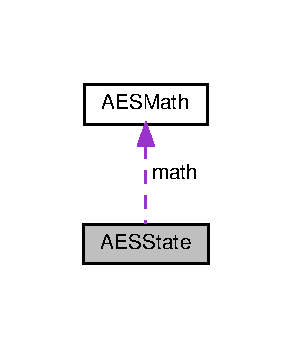
\includegraphics[width=140pt]{classAESState__coll__graph}
\end{center}
\end{figure}
\subsection*{Public Member Functions}
\begin{DoxyCompactItemize}
\item 
\mbox{\Hypertarget{classAESState_a2cc9414a52e4f828dce31db66af44f12}\label{classAESState_a2cc9414a52e4f828dce31db66af44f12}} 
{\bfseries A\+E\+S\+State} (const \hyperlink{classAESMath}{A\+E\+S\+Math} \&aesmath, bool debug\+\_\+mode=false)
\item 
\mbox{\Hypertarget{classAESState_a289634d47fcbde24b1464c8b82ee04f5}\label{classAESState_a289634d47fcbde24b1464c8b82ee04f5}} 
void {\bfseries set} (const byte $\ast$in)
\item 
\mbox{\Hypertarget{classAESState_a374f83c433060db458a586923b2aa116}\label{classAESState_a374f83c433060db458a586923b2aa116}} 
void {\bfseries get} (byte $\ast$out)
\item 
\mbox{\Hypertarget{classAESState_aed74abc14779f7d8fcbfea6f06649640}\label{classAESState_aed74abc14779f7d8fcbfea6f06649640}} 
void {\bfseries shift\+Rows} ()
\item 
\mbox{\Hypertarget{classAESState_ab18b4607210ae88bd825e7b9ca4529a6}\label{classAESState_ab18b4607210ae88bd825e7b9ca4529a6}} 
void {\bfseries sub\+Bytes} ()
\item 
\mbox{\Hypertarget{classAESState_a88494d311817ef8ac87984fdc475b138}\label{classAESState_a88494d311817ef8ac87984fdc475b138}} 
void {\bfseries mix\+Columns} ()
\item 
\mbox{\Hypertarget{classAESState_a08dcc6810da02059f3dea7ef0ad50a8e}\label{classAESState_a08dcc6810da02059f3dea7ef0ad50a8e}} 
void {\bfseries inv\+Shift\+Rows} ()
\item 
\mbox{\Hypertarget{classAESState_abfa9f233a7776649ac044d581f88f240}\label{classAESState_abfa9f233a7776649ac044d581f88f240}} 
void {\bfseries inv\+Sub\+Bytes} ()
\item 
\mbox{\Hypertarget{classAESState_a5a16a03a1569836f8876d9822e8d3874}\label{classAESState_a5a16a03a1569836f8876d9822e8d3874}} 
void {\bfseries inv\+Mix\+Columns} ()
\item 
\mbox{\Hypertarget{classAESState_abdd8d914886e56653c5a78d3605abf1d}\label{classAESState_abdd8d914886e56653c5a78d3605abf1d}} 
void {\bfseries add\+Key} (const word $\ast$key)
\item 
\mbox{\Hypertarget{classAESState_a968bcb473d9dfb281f9d753d621792c9}\label{classAESState_a968bcb473d9dfb281f9d753d621792c9}} 
string {\bfseries format} () const
\end{DoxyCompactItemize}
\subsection*{Protected Member Functions}
\begin{DoxyCompactItemize}
\item 
\mbox{\Hypertarget{classAESState_a40b1c825513553815de61e1f8e2b89be}\label{classAESState_a40b1c825513553815de61e1f8e2b89be}} 
byte {\bfseries get\+Cell} (size\+\_\+t row, size\+\_\+t col)
\item 
\mbox{\Hypertarget{classAESState_a8fc413a6fdf8211a8c81341c5fb98b2f}\label{classAESState_a8fc413a6fdf8211a8c81341c5fb98b2f}} 
void {\bfseries set\+Cell} (size\+\_\+t row, size\+\_\+t col, byte b)
\item 
\mbox{\Hypertarget{classAESState_ad0b0ce9b90a20e90ebe714a96cb0513c}\label{classAESState_ad0b0ce9b90a20e90ebe714a96cb0513c}} 
void {\bfseries shift\+Row} (size\+\_\+t row, size\+\_\+t shift)
\end{DoxyCompactItemize}
\subsection*{Protected Attributes}
\begin{DoxyCompactItemize}
\item 
\mbox{\Hypertarget{classAESState_a0ecd8ba384844aec6e8ad93b9ad1477b}\label{classAESState_a0ecd8ba384844aec6e8ad93b9ad1477b}} 
byte {\bfseries state} \mbox{[}16\mbox{]}
\end{DoxyCompactItemize}
\subsection*{Private Attributes}
\begin{DoxyCompactItemize}
\item 
\mbox{\Hypertarget{classAESState_a7cd68a8ad4ea900df93a9adca4531a04}\label{classAESState_a7cd68a8ad4ea900df93a9adca4531a04}} 
bool {\bfseries debug\+\_\+mode}
\item 
\mbox{\Hypertarget{classAESState_afd42377ff30e9d15bfef8a09e768380e}\label{classAESState_afd42377ff30e9d15bfef8a09e768380e}} 
const \hyperlink{classAESMath}{A\+E\+S\+Math} $\ast$ {\bfseries math}
\end{DoxyCompactItemize}


The documentation for this class was generated from the following files\+:\begin{DoxyCompactItemize}
\item 
/home/sinflair/\+P/crypto/\+A\+K/src/\+Praktikum-\/\+A\+E\+S/A\+E\+S\+State.\+h\item 
/home/sinflair/\+P/crypto/\+A\+K/src/\+Praktikum-\/\+A\+E\+S/A\+E\+S\+State.\+cpp\end{DoxyCompactItemize}

\hypertarget{classBlockCipher}{}\section{Block\+Cipher Class Reference}
\label{classBlockCipher}\index{Block\+Cipher@{Block\+Cipher}}


Inheritance diagram for Block\+Cipher\+:
\nopagebreak
\begin{figure}[H]
\begin{center}
\leavevmode
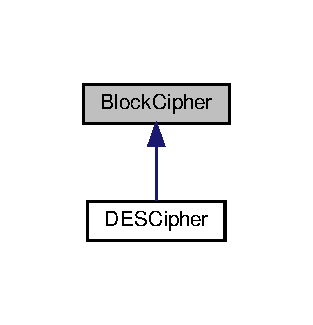
\includegraphics[width=150pt]{classBlockCipher__inherit__graph}
\end{center}
\end{figure}
\subsection*{Public Member Functions}
\begin{DoxyCompactItemize}
\item 
\mbox{\Hypertarget{classBlockCipher_a3c95996f1004e8bbf2b681168d1bd0a9}\label{classBlockCipher_a3c95996f1004e8bbf2b681168d1bd0a9}} 
{\bfseries Block\+Cipher} (unsigned int in\+\_\+block\+\_\+len=8)
\item 
\mbox{\Hypertarget{classBlockCipher_aa6feefe4bf7b8844c44e06240439715a}\label{classBlockCipher_aa6feefe4bf7b8844c44e06240439715a}} 
virtual bool {\bfseries decrypt} (const vector$<$ byte $>$ \&plain\+\_\+text, vector$<$ byte $>$ \&cipher\+\_\+text)=0
\item 
\mbox{\Hypertarget{classBlockCipher_a6b9e82d14004c855a47d79e9de8b3450}\label{classBlockCipher_a6b9e82d14004c855a47d79e9de8b3450}} 
virtual bool {\bfseries encrypt} (const vector$<$ byte $>$ \&plain\+\_\+text, vector$<$ byte $>$ \&cipher\+\_\+text)=0
\item 
\mbox{\Hypertarget{classBlockCipher_a2d97a0cb8efa9109eefea09c7019f064}\label{classBlockCipher_a2d97a0cb8efa9109eefea09c7019f064}} 
virtual bool {\bfseries set\+Key} (const vector$<$ byte $>$ \&key)=0
\end{DoxyCompactItemize}
\subsection*{Static Public Member Functions}
\begin{DoxyCompactItemize}
\item 
\mbox{\Hypertarget{classBlockCipher_ae55a65434bf1d4b59375916a0e58664c}\label{classBlockCipher_ae55a65434bf1d4b59375916a0e58664c}} 
static byte {\bfseries hex\+To\+Byte} (byte xdigit)
\item 
\mbox{\Hypertarget{classBlockCipher_a6c951af389b9ddb9f40c410d18ab5c66}\label{classBlockCipher_a6c951af389b9ddb9f40c410d18ab5c66}} 
static bool {\bfseries read\+Stream} (istream \&strm, vector$<$ byte $>$ \&data, bool hex\+\_\+mode)
\item 
\mbox{\Hypertarget{classBlockCipher_a3839442ae65dd2a710a015b53e9117bf}\label{classBlockCipher_a3839442ae65dd2a710a015b53e9117bf}} 
static void {\bfseries write\+Stream} (ostream \&strm, const vector$<$ byte $>$ \&data, bool hex\+\_\+mode, int columns=30)
\item 
\mbox{\Hypertarget{classBlockCipher_a58dfa6f0548071b3988c8c8990e54c93}\label{classBlockCipher_a58dfa6f0548071b3988c8c8990e54c93}} 
static bool {\bfseries hex\+String\+To\+Vector} (string s, vector$<$ byte $>$ \&data)
\item 
\mbox{\Hypertarget{classBlockCipher_ad000d34ae66e52ee8484a651793d7dfa}\label{classBlockCipher_ad000d34ae66e52ee8484a651793d7dfa}} 
static string {\bfseries to\+Hex\+String} (const vector$<$ byte $>$ \&data)
\end{DoxyCompactItemize}
\subsection*{Protected Attributes}
\begin{DoxyCompactItemize}
\item 
\mbox{\Hypertarget{classBlockCipher_ab29ee03262fd620cd0659e860972faf0}\label{classBlockCipher_ab29ee03262fd620cd0659e860972faf0}} 
unsigned int {\bfseries block\+\_\+len}
\end{DoxyCompactItemize}


The documentation for this class was generated from the following files\+:\begin{DoxyCompactItemize}
\item 
/home/sinflair/\+P/crypto/\+A\+K/src/\+Praktikum-\/\+A\+E\+S/Block\+Cipher.\+h\item 
/home/sinflair/\+P/crypto/\+A\+K/src/\+Praktikum-\/\+A\+E\+S/Block\+Cipher.\+cpp\end{DoxyCompactItemize}

\hypertarget{structcmdline__parser__params}{}\section{cmdline\+\_\+parser\+\_\+params Struct Reference}
\label{structcmdline__parser__params}\index{cmdline\+\_\+parser\+\_\+params@{cmdline\+\_\+parser\+\_\+params}}


The additional parameters to pass to parser functions.  




{\ttfamily \#include $<$aes-\/getopt.\+h$>$}

\subsection*{Public Attributes}
\begin{DoxyCompactItemize}
\item 
\mbox{\Hypertarget{structcmdline__parser__params_ad3ff9d69146e69a47506782197b5675c}\label{structcmdline__parser__params_ad3ff9d69146e69a47506782197b5675c}} 
int \hyperlink{structcmdline__parser__params_ad3ff9d69146e69a47506782197b5675c}{override}
\begin{DoxyCompactList}\small\item\em whether to override possibly already present options (default 0) \end{DoxyCompactList}\item 
\mbox{\Hypertarget{structcmdline__parser__params_a97ed8a6eabd39291ae7d73f273e12c11}\label{structcmdline__parser__params_a97ed8a6eabd39291ae7d73f273e12c11}} 
int \hyperlink{structcmdline__parser__params_a97ed8a6eabd39291ae7d73f273e12c11}{initialize}
\begin{DoxyCompactList}\small\item\em whether to initialize the option structure \hyperlink{structgengetopt__args__info}{gengetopt\+\_\+args\+\_\+info} (default 1) \end{DoxyCompactList}\item 
\mbox{\Hypertarget{structcmdline__parser__params_a44ff439d7e9e36799e59173af74829c6}\label{structcmdline__parser__params_a44ff439d7e9e36799e59173af74829c6}} 
int \hyperlink{structcmdline__parser__params_a44ff439d7e9e36799e59173af74829c6}{check\+\_\+required}
\begin{DoxyCompactList}\small\item\em whether to check that all required options were provided (default 1) \end{DoxyCompactList}\item 
\mbox{\Hypertarget{structcmdline__parser__params_a6e4442704fc40b0b655f7cc602f13ec4}\label{structcmdline__parser__params_a6e4442704fc40b0b655f7cc602f13ec4}} 
int \hyperlink{structcmdline__parser__params_a6e4442704fc40b0b655f7cc602f13ec4}{check\+\_\+ambiguity}
\begin{DoxyCompactList}\small\item\em whether to check for options already specified in the option structure \hyperlink{structgengetopt__args__info}{gengetopt\+\_\+args\+\_\+info} (default 0) \end{DoxyCompactList}\item 
\mbox{\Hypertarget{structcmdline__parser__params_a3236f066777488e8502abe05ccd24455}\label{structcmdline__parser__params_a3236f066777488e8502abe05ccd24455}} 
int \hyperlink{structcmdline__parser__params_a3236f066777488e8502abe05ccd24455}{print\+\_\+errors}
\begin{DoxyCompactList}\small\item\em whether getopt\+\_\+long should print an error message for a bad option (default 1) \end{DoxyCompactList}\end{DoxyCompactItemize}


\subsection{Detailed Description}
The additional parameters to pass to parser functions. 

The documentation for this struct was generated from the following file\+:\begin{DoxyCompactItemize}
\item 
/home/sinflair/\+P/crypto/\+A\+K/src/\+Praktikum-\/\+A\+E\+S/\hyperlink{aes-getopt_8h}{aes-\/getopt.\+h}\end{DoxyCompactItemize}

\hypertarget{structcustom__getopt__data}{}\section{custom\+\_\+getopt\+\_\+data Struct Reference}
\label{structcustom__getopt__data}\index{custom\+\_\+getopt\+\_\+data@{custom\+\_\+getopt\+\_\+data}}
\subsection*{Public Attributes}
\begin{DoxyCompactItemize}
\item 
\mbox{\Hypertarget{structcustom__getopt__data_a708838699338a902634d6040f61c9d1e}\label{structcustom__getopt__data_a708838699338a902634d6040f61c9d1e}} 
int {\bfseries custom\+\_\+optind}
\item 
\mbox{\Hypertarget{structcustom__getopt__data_a70368029b9189c6af100d41b95a2a853}\label{structcustom__getopt__data_a70368029b9189c6af100d41b95a2a853}} 
int {\bfseries custom\+\_\+opterr}
\item 
\mbox{\Hypertarget{structcustom__getopt__data_ad986661b4b79755fd55f9f10303221e0}\label{structcustom__getopt__data_ad986661b4b79755fd55f9f10303221e0}} 
int {\bfseries custom\+\_\+optopt}
\item 
\mbox{\Hypertarget{structcustom__getopt__data_a09e50973b9ce49fa0bfa62bb06289f32}\label{structcustom__getopt__data_a09e50973b9ce49fa0bfa62bb06289f32}} 
char $\ast$ {\bfseries custom\+\_\+optarg}
\item 
\mbox{\Hypertarget{structcustom__getopt__data_a5952791becb49374ddfc8726bbf94910}\label{structcustom__getopt__data_a5952791becb49374ddfc8726bbf94910}} 
int {\bfseries initialized}
\item 
\mbox{\Hypertarget{structcustom__getopt__data_a83f042e31dab41b17d8238b528e06121}\label{structcustom__getopt__data_a83f042e31dab41b17d8238b528e06121}} 
char $\ast$ {\bfseries nextchar}
\item 
\mbox{\Hypertarget{structcustom__getopt__data_a89f56362160b74f59aa39d8838dd8bb8}\label{structcustom__getopt__data_a89f56362160b74f59aa39d8838dd8bb8}} 
int {\bfseries first\+\_\+nonopt}
\item 
\mbox{\Hypertarget{structcustom__getopt__data_aff78193409ca6ea017ced550453e0cfd}\label{structcustom__getopt__data_aff78193409ca6ea017ced550453e0cfd}} 
int {\bfseries last\+\_\+nonopt}
\end{DoxyCompactItemize}


The documentation for this struct was generated from the following file\+:\begin{DoxyCompactItemize}
\item 
/home/sinflair/\+P/crypto/\+A\+K/src/\+Praktikum-\/\+A\+E\+S/aes-\/getopt.\+c\end{DoxyCompactItemize}

\hypertarget{structgengetopt__args__info}{}\section{gengetopt\+\_\+args\+\_\+info Struct Reference}
\label{structgengetopt__args__info}\index{gengetopt\+\_\+args\+\_\+info@{gengetopt\+\_\+args\+\_\+info}}


Where the command line options are stored.  




{\ttfamily \#include $<$aes-\/getopt.\+h$>$}

\subsection*{Public Attributes}
\begin{DoxyCompactItemize}
\item 
\mbox{\Hypertarget{structgengetopt__args__info_afb4efa68a6f43a4d112e9b96ffe89101}\label{structgengetopt__args__info_afb4efa68a6f43a4d112e9b96ffe89101}} 
const char $\ast$ \hyperlink{structgengetopt__args__info_afb4efa68a6f43a4d112e9b96ffe89101}{help\+\_\+help}
\begin{DoxyCompactList}\small\item\em Print help and exit help description. \end{DoxyCompactList}\item 
\mbox{\Hypertarget{structgengetopt__args__info_adef454ea6f3ff4114ae5009e58360cfc}\label{structgengetopt__args__info_adef454ea6f3ff4114ae5009e58360cfc}} 
const char $\ast$ \hyperlink{structgengetopt__args__info_adef454ea6f3ff4114ae5009e58360cfc}{version\+\_\+help}
\begin{DoxyCompactList}\small\item\em Print version and exit help description. \end{DoxyCompactList}\item 
\mbox{\Hypertarget{structgengetopt__args__info_a9d2e2cfeae6c1b4644a9e539dd37b490}\label{structgengetopt__args__info_a9d2e2cfeae6c1b4644a9e539dd37b490}} 
char $\ast$ \hyperlink{structgengetopt__args__info_a9d2e2cfeae6c1b4644a9e539dd37b490}{key\+\_\+arg}
\begin{DoxyCompactList}\small\item\em Key to be used for encryption or decryption. \end{DoxyCompactList}\item 
\mbox{\Hypertarget{structgengetopt__args__info_a46fe55fd04263db7ebf4d5afa09f696f}\label{structgengetopt__args__info_a46fe55fd04263db7ebf4d5afa09f696f}} 
char $\ast$ \hyperlink{structgengetopt__args__info_a46fe55fd04263db7ebf4d5afa09f696f}{key\+\_\+orig}
\begin{DoxyCompactList}\small\item\em Key to be used for encryption or decryption original value given at command line. \end{DoxyCompactList}\item 
\mbox{\Hypertarget{structgengetopt__args__info_a9f98c455fbbd65117dbbd1e17723c92e}\label{structgengetopt__args__info_a9f98c455fbbd65117dbbd1e17723c92e}} 
const char $\ast$ \hyperlink{structgengetopt__args__info_a9f98c455fbbd65117dbbd1e17723c92e}{key\+\_\+help}
\begin{DoxyCompactList}\small\item\em Key to be used for encryption or decryption help description. \end{DoxyCompactList}\item 
\mbox{\Hypertarget{structgengetopt__args__info_a1022ab6bd8cfa9596789a6a7059be6af}\label{structgengetopt__args__info_a1022ab6bd8cfa9596789a6a7059be6af}} 
char $\ast$ \hyperlink{structgengetopt__args__info_a1022ab6bd8cfa9596789a6a7059be6af}{out\+\_\+arg}
\begin{DoxyCompactList}\small\item\em output file. \end{DoxyCompactList}\item 
\mbox{\Hypertarget{structgengetopt__args__info_a342bcb7cbcac1cbaefd3ffaafa3736ff}\label{structgengetopt__args__info_a342bcb7cbcac1cbaefd3ffaafa3736ff}} 
char $\ast$ \hyperlink{structgengetopt__args__info_a342bcb7cbcac1cbaefd3ffaafa3736ff}{out\+\_\+orig}
\begin{DoxyCompactList}\small\item\em output file original value given at command line. \end{DoxyCompactList}\item 
\mbox{\Hypertarget{structgengetopt__args__info_ad1e0068ecb61c96fc1b239c575d125d9}\label{structgengetopt__args__info_ad1e0068ecb61c96fc1b239c575d125d9}} 
const char $\ast$ \hyperlink{structgengetopt__args__info_ad1e0068ecb61c96fc1b239c575d125d9}{out\+\_\+help}
\begin{DoxyCompactList}\small\item\em output file help description. \end{DoxyCompactList}\item 
\mbox{\Hypertarget{structgengetopt__args__info_a31a0c7c5b907732c8f4f74717bfdb8bc}\label{structgengetopt__args__info_a31a0c7c5b907732c8f4f74717bfdb8bc}} 
const char $\ast$ \hyperlink{structgengetopt__args__info_a31a0c7c5b907732c8f4f74717bfdb8bc}{encrypt\+\_\+help}
\begin{DoxyCompactList}\small\item\em Encryption help description. \end{DoxyCompactList}\item 
\mbox{\Hypertarget{structgengetopt__args__info_a1e9e71d6f662ce2a1eef16dd13f18ef4}\label{structgengetopt__args__info_a1e9e71d6f662ce2a1eef16dd13f18ef4}} 
const char $\ast$ \hyperlink{structgengetopt__args__info_a1e9e71d6f662ce2a1eef16dd13f18ef4}{decrypt\+\_\+help}
\begin{DoxyCompactList}\small\item\em Decryption help description. \end{DoxyCompactList}\item 
\mbox{\Hypertarget{structgengetopt__args__info_ab9fd677f890731fd7d6f6c62e6dfc99c}\label{structgengetopt__args__info_ab9fd677f890731fd7d6f6c62e6dfc99c}} 
unsigned int \hyperlink{structgengetopt__args__info_ab9fd677f890731fd7d6f6c62e6dfc99c}{help\+\_\+given}
\begin{DoxyCompactList}\small\item\em Whether help was given. \end{DoxyCompactList}\item 
\mbox{\Hypertarget{structgengetopt__args__info_ad4953a2130b2f8b94a3a687014f278e1}\label{structgengetopt__args__info_ad4953a2130b2f8b94a3a687014f278e1}} 
unsigned int \hyperlink{structgengetopt__args__info_ad4953a2130b2f8b94a3a687014f278e1}{version\+\_\+given}
\begin{DoxyCompactList}\small\item\em Whether version was given. \end{DoxyCompactList}\item 
\mbox{\Hypertarget{structgengetopt__args__info_a155a1a709ea64f935a0cda6ebe932f33}\label{structgengetopt__args__info_a155a1a709ea64f935a0cda6ebe932f33}} 
unsigned int \hyperlink{structgengetopt__args__info_a155a1a709ea64f935a0cda6ebe932f33}{key\+\_\+given}
\begin{DoxyCompactList}\small\item\em Whether key was given. \end{DoxyCompactList}\item 
\mbox{\Hypertarget{structgengetopt__args__info_a0b95b56ea8bfba9d7d1dfc92a1ba8feb}\label{structgengetopt__args__info_a0b95b56ea8bfba9d7d1dfc92a1ba8feb}} 
unsigned int \hyperlink{structgengetopt__args__info_a0b95b56ea8bfba9d7d1dfc92a1ba8feb}{out\+\_\+given}
\begin{DoxyCompactList}\small\item\em Whether out was given. \end{DoxyCompactList}\item 
\mbox{\Hypertarget{structgengetopt__args__info_a2cc94a70a7e771ee78c947d08dd8cf1d}\label{structgengetopt__args__info_a2cc94a70a7e771ee78c947d08dd8cf1d}} 
unsigned int \hyperlink{structgengetopt__args__info_a2cc94a70a7e771ee78c947d08dd8cf1d}{encrypt\+\_\+given}
\begin{DoxyCompactList}\small\item\em Whether encrypt was given. \end{DoxyCompactList}\item 
\mbox{\Hypertarget{structgengetopt__args__info_ab8fb4a2ce4915d98294802d3b361325f}\label{structgengetopt__args__info_ab8fb4a2ce4915d98294802d3b361325f}} 
unsigned int \hyperlink{structgengetopt__args__info_ab8fb4a2ce4915d98294802d3b361325f}{decrypt\+\_\+given}
\begin{DoxyCompactList}\small\item\em Whether decrypt was given. \end{DoxyCompactList}\item 
\mbox{\Hypertarget{structgengetopt__args__info_a9604690019dd09b318302dae6868726c}\label{structgengetopt__args__info_a9604690019dd09b318302dae6868726c}} 
char $\ast$$\ast$ \hyperlink{structgengetopt__args__info_a9604690019dd09b318302dae6868726c}{inputs}
\begin{DoxyCompactList}\small\item\em unamed options (options without names) \end{DoxyCompactList}\item 
\mbox{\Hypertarget{structgengetopt__args__info_a3d69c180d5ac0b1124fd9a6fe680706c}\label{structgengetopt__args__info_a3d69c180d5ac0b1124fd9a6fe680706c}} 
unsigned \hyperlink{structgengetopt__args__info_a3d69c180d5ac0b1124fd9a6fe680706c}{inputs\+\_\+num}
\begin{DoxyCompactList}\small\item\em unamed options number \end{DoxyCompactList}\item 
\mbox{\Hypertarget{structgengetopt__args__info_a44f277219c706b8ca8b64ce3d9f3f2ec}\label{structgengetopt__args__info_a44f277219c706b8ca8b64ce3d9f3f2ec}} 
int \hyperlink{structgengetopt__args__info_a44f277219c706b8ca8b64ce3d9f3f2ec}{opmode\+\_\+group\+\_\+counter}
\begin{DoxyCompactList}\small\item\em Counter for group opmode. \end{DoxyCompactList}\end{DoxyCompactItemize}


\subsection{Detailed Description}
Where the command line options are stored. 

The documentation for this struct was generated from the following file\+:\begin{DoxyCompactItemize}
\item 
/home/sinflair/\+P/crypto/\+A\+K/src/\+Praktikum-\/\+A\+E\+S/\hyperlink{aes-getopt_8h}{aes-\/getopt.\+h}\end{DoxyCompactItemize}

\hypertarget{structoption}{}\section{option Struct Reference}
\label{structoption}\index{option@{option}}
\subsection*{Public Attributes}
\begin{DoxyCompactItemize}
\item 
\mbox{\Hypertarget{structoption_adc503659d37af8017fb4b86d61c99086}\label{structoption_adc503659d37af8017fb4b86d61c99086}} 
const char $\ast$ {\bfseries name}
\item 
\mbox{\Hypertarget{structoption_a90d7ee9a51eea5c002682dbd0af149e4}\label{structoption_a90d7ee9a51eea5c002682dbd0af149e4}} 
int {\bfseries has\+\_\+arg}
\item 
\mbox{\Hypertarget{structoption_ab366eea5fe7be25c1928328ba715e353}\label{structoption_ab366eea5fe7be25c1928328ba715e353}} 
int $\ast$ {\bfseries flag}
\item 
\mbox{\Hypertarget{structoption_a13bd155ec3b405d29c41ab8d0793be11}\label{structoption_a13bd155ec3b405d29c41ab8d0793be11}} 
int {\bfseries val}
\end{DoxyCompactItemize}


The documentation for this struct was generated from the following file\+:\begin{DoxyCompactItemize}
\item 
/home/sinflair/\+P/crypto/\+A\+K/src/\+Praktikum-\/\+A\+E\+S/aes-\/getopt.\+c\end{DoxyCompactItemize}

\chapter{File Documentation}
\hypertarget{aes-getopt_8h}{}\section{/home/sinflair/\+P/crypto/\+A\+K/src/\+Praktikum-\/\+A\+E\+S/aes-\/getopt.h File Reference}
\label{aes-getopt_8h}\index{/home/sinflair/\+P/crypto/\+A\+K/src/\+Praktikum-\/\+A\+E\+S/aes-\/getopt.\+h@{/home/sinflair/\+P/crypto/\+A\+K/src/\+Praktikum-\/\+A\+E\+S/aes-\/getopt.\+h}}


The header file for the command line option parser generated by G\+NU Gengetopt version 2.\+22.\+6 \href{http://www.gnu.org/software/gengetopt}{\tt http\+://www.\+gnu.\+org/software/gengetopt}. DO N\+OT modify this file, since it can be overwritten.  


{\ttfamily \#include $<$stdio.\+h$>$}\newline
Include dependency graph for aes-\/getopt.h\+:
\nopagebreak
\begin{figure}[H]
\begin{center}
\leavevmode
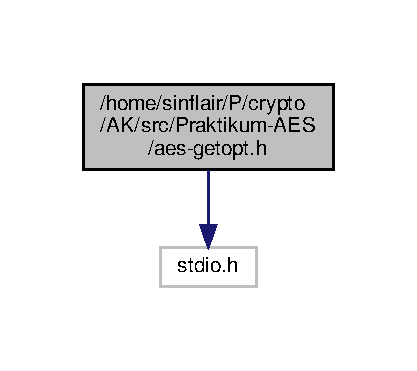
\includegraphics[width=200pt]{aes-getopt_8h__incl}
\end{center}
\end{figure}
\subsection*{Classes}
\begin{DoxyCompactItemize}
\item 
struct \hyperlink{structgengetopt__args__info}{gengetopt\+\_\+args\+\_\+info}
\begin{DoxyCompactList}\small\item\em Where the command line options are stored. \end{DoxyCompactList}\item 
struct \hyperlink{structcmdline__parser__params}{cmdline\+\_\+parser\+\_\+params}
\begin{DoxyCompactList}\small\item\em The additional parameters to pass to parser functions. \end{DoxyCompactList}\end{DoxyCompactItemize}
\subsection*{Macros}
\begin{DoxyCompactItemize}
\item 
\mbox{\Hypertarget{aes-getopt_8h_aeb847973552c32bcbe5f14973a0a8a32}\label{aes-getopt_8h_aeb847973552c32bcbe5f14973a0a8a32}} 
\#define \hyperlink{aes-getopt_8h_aeb847973552c32bcbe5f14973a0a8a32}{C\+M\+D\+L\+I\+N\+E\+\_\+\+P\+A\+R\+S\+E\+R\+\_\+\+P\+A\+C\+K\+A\+GE}~\char`\"{}des\char`\"{}
\begin{DoxyCompactList}\small\item\em the program name (used for printing errors) \end{DoxyCompactList}\item 
\mbox{\Hypertarget{aes-getopt_8h_ae2f94765d0d8758ddf6b326a4806d6ff}\label{aes-getopt_8h_ae2f94765d0d8758ddf6b326a4806d6ff}} 
\#define \hyperlink{aes-getopt_8h_ae2f94765d0d8758ddf6b326a4806d6ff}{C\+M\+D\+L\+I\+N\+E\+\_\+\+P\+A\+R\+S\+E\+R\+\_\+\+P\+A\+C\+K\+A\+G\+E\+\_\+\+N\+A\+ME}~\char`\"{}des\char`\"{}
\begin{DoxyCompactList}\small\item\em the complete program name (used for help and version) \end{DoxyCompactList}\item 
\mbox{\Hypertarget{aes-getopt_8h_a1eeca7dc254bf6867ba9635f45771471}\label{aes-getopt_8h_a1eeca7dc254bf6867ba9635f45771471}} 
\#define \hyperlink{aes-getopt_8h_a1eeca7dc254bf6867ba9635f45771471}{C\+M\+D\+L\+I\+N\+E\+\_\+\+P\+A\+R\+S\+E\+R\+\_\+\+V\+E\+R\+S\+I\+ON}~\char`\"{}0.\+0.\+1\char`\"{}
\begin{DoxyCompactList}\small\item\em the program version \end{DoxyCompactList}\end{DoxyCompactItemize}
\subsection*{Functions}
\begin{DoxyCompactItemize}
\item 
int \hyperlink{aes-getopt_8h_a3c3df73307452c51fee0a34640d92196}{cmdline\+\_\+parser} (int argc, char $\ast$$\ast$argv, struct \hyperlink{structgengetopt__args__info}{gengetopt\+\_\+args\+\_\+info} $\ast$args\+\_\+info)
\item 
int \hyperlink{aes-getopt_8h_a78a0cd581698415a62f68214603b1a30}{cmdline\+\_\+parser2} (int argc, char $\ast$$\ast$argv, struct \hyperlink{structgengetopt__args__info}{gengetopt\+\_\+args\+\_\+info} $\ast$args\+\_\+info, int override, int initialize, int check\+\_\+required)
\item 
int \hyperlink{aes-getopt_8h_ac7bb5d76f3f56d1c0b3b531f11ac6f07}{cmdline\+\_\+parser\+\_\+ext} (int argc, char $\ast$$\ast$argv, struct \hyperlink{structgengetopt__args__info}{gengetopt\+\_\+args\+\_\+info} $\ast$args\+\_\+info, struct \hyperlink{structcmdline__parser__params}{cmdline\+\_\+parser\+\_\+params} $\ast$params)
\item 
int \hyperlink{aes-getopt_8h_a1f73418092a6e6eb3706aa0de2785e11}{cmdline\+\_\+parser\+\_\+dump} (F\+I\+LE $\ast$outfile, struct \hyperlink{structgengetopt__args__info}{gengetopt\+\_\+args\+\_\+info} $\ast$args\+\_\+info)
\item 
int \hyperlink{aes-getopt_8h_a5f3e9412f88f1058a31ac28ad2ea2818}{cmdline\+\_\+parser\+\_\+file\+\_\+save} (const char $\ast$filename, struct \hyperlink{structgengetopt__args__info}{gengetopt\+\_\+args\+\_\+info} $\ast$args\+\_\+info)
\item 
void \hyperlink{aes-getopt_8h_ad4f7db2fa4002379eb30e5206f3b7492}{cmdline\+\_\+parser\+\_\+print\+\_\+help} (void)
\item 
void \hyperlink{aes-getopt_8h_a96f27bf35ce0ab8eea7a1f6e6b59a5e2}{cmdline\+\_\+parser\+\_\+print\+\_\+version} (void)
\item 
void \hyperlink{aes-getopt_8h_af72b814611cffc706b2135ccdfe7e997}{cmdline\+\_\+parser\+\_\+params\+\_\+init} (struct \hyperlink{structcmdline__parser__params}{cmdline\+\_\+parser\+\_\+params} $\ast$params)
\item 
struct \hyperlink{structcmdline__parser__params}{cmdline\+\_\+parser\+\_\+params} $\ast$ \hyperlink{aes-getopt_8h_afd778af110fe0ee1ea5eac7aa9939d92}{cmdline\+\_\+parser\+\_\+params\+\_\+create} (void)
\item 
void \hyperlink{aes-getopt_8h_aca62b50d03d0d082968eeb1940f98650}{cmdline\+\_\+parser\+\_\+init} (struct \hyperlink{structgengetopt__args__info}{gengetopt\+\_\+args\+\_\+info} $\ast$args\+\_\+info)
\item 
void \hyperlink{aes-getopt_8h_af1b97c4e92b88f736e350b3902266ba4}{cmdline\+\_\+parser\+\_\+free} (struct \hyperlink{structgengetopt__args__info}{gengetopt\+\_\+args\+\_\+info} $\ast$args\+\_\+info)
\item 
int \hyperlink{aes-getopt_8h_a83651e5be280d60aed58fdb72456a030}{cmdline\+\_\+parser\+\_\+required} (struct \hyperlink{structgengetopt__args__info}{gengetopt\+\_\+args\+\_\+info} $\ast$args\+\_\+info, const char $\ast$prog\+\_\+name)
\end{DoxyCompactItemize}
\subsection*{Variables}
\begin{DoxyCompactItemize}
\item 
\mbox{\Hypertarget{aes-getopt_8h_a610c3307abce5a8fd304b86b018ae60b}\label{aes-getopt_8h_a610c3307abce5a8fd304b86b018ae60b}} 
const char $\ast$ \hyperlink{aes-getopt_8h_a610c3307abce5a8fd304b86b018ae60b}{gengetopt\+\_\+args\+\_\+info\+\_\+purpose}
\begin{DoxyCompactList}\small\item\em the purpose string of the program \end{DoxyCompactList}\item 
\mbox{\Hypertarget{aes-getopt_8h_a9f397a306f363bfdebb611e86acf36d5}\label{aes-getopt_8h_a9f397a306f363bfdebb611e86acf36d5}} 
const char $\ast$ \hyperlink{aes-getopt_8h_a9f397a306f363bfdebb611e86acf36d5}{gengetopt\+\_\+args\+\_\+info\+\_\+usage}
\begin{DoxyCompactList}\small\item\em the usage string of the program \end{DoxyCompactList}\item 
\mbox{\Hypertarget{aes-getopt_8h_accad6107ca685f6eba555f6ce63d355d}\label{aes-getopt_8h_accad6107ca685f6eba555f6ce63d355d}} 
const char $\ast$ \hyperlink{aes-getopt_8h_accad6107ca685f6eba555f6ce63d355d}{gengetopt\+\_\+args\+\_\+info\+\_\+description}
\begin{DoxyCompactList}\small\item\em the description string of the program \end{DoxyCompactList}\item 
\mbox{\Hypertarget{aes-getopt_8h_a6af7a6b7fb37c0abaa916ee1cfa0a41f}\label{aes-getopt_8h_a6af7a6b7fb37c0abaa916ee1cfa0a41f}} 
const char $\ast$ \hyperlink{aes-getopt_8h_a6af7a6b7fb37c0abaa916ee1cfa0a41f}{gengetopt\+\_\+args\+\_\+info\+\_\+help} \mbox{[}$\,$\mbox{]}
\begin{DoxyCompactList}\small\item\em all the lines making the help output \end{DoxyCompactList}\end{DoxyCompactItemize}


\subsection{Detailed Description}
The header file for the command line option parser generated by G\+NU Gengetopt version 2.\+22.\+6 \href{http://www.gnu.org/software/gengetopt}{\tt http\+://www.\+gnu.\+org/software/gengetopt}. DO N\+OT modify this file, since it can be overwritten. 

\begin{DoxyAuthor}{Author}
G\+NU Gengetopt by Lorenzo Bettini 
\end{DoxyAuthor}


\subsection{Function Documentation}
\mbox{\Hypertarget{aes-getopt_8h_a3c3df73307452c51fee0a34640d92196}\label{aes-getopt_8h_a3c3df73307452c51fee0a34640d92196}} 
\index{aes-\/getopt.\+h@{aes-\/getopt.\+h}!cmdline\+\_\+parser@{cmdline\+\_\+parser}}
\index{cmdline\+\_\+parser@{cmdline\+\_\+parser}!aes-\/getopt.\+h@{aes-\/getopt.\+h}}
\subsubsection{\texorpdfstring{cmdline\+\_\+parser()}{cmdline\_parser()}}
{\footnotesize\ttfamily int cmdline\+\_\+parser (\begin{DoxyParamCaption}\item[{int}]{argc,  }\item[{char $\ast$$\ast$}]{argv,  }\item[{struct \hyperlink{structgengetopt__args__info}{gengetopt\+\_\+args\+\_\+info} $\ast$}]{args\+\_\+info }\end{DoxyParamCaption})}

The command line parser 
\begin{DoxyParams}{Parameters}
{\em argc} & the number of command line options \\
\hline
{\em argv} & the command line options \\
\hline
{\em args\+\_\+info} & the structure where option information will be stored \\
\hline
\end{DoxyParams}
\begin{DoxyReturn}{Returns}
0 if everything went fine, N\+ON 0 if an error took place 
\end{DoxyReturn}
\mbox{\Hypertarget{aes-getopt_8h_a78a0cd581698415a62f68214603b1a30}\label{aes-getopt_8h_a78a0cd581698415a62f68214603b1a30}} 
\index{aes-\/getopt.\+h@{aes-\/getopt.\+h}!cmdline\+\_\+parser2@{cmdline\+\_\+parser2}}
\index{cmdline\+\_\+parser2@{cmdline\+\_\+parser2}!aes-\/getopt.\+h@{aes-\/getopt.\+h}}
\subsubsection{\texorpdfstring{cmdline\+\_\+parser2()}{cmdline\_parser2()}}
{\footnotesize\ttfamily int cmdline\+\_\+parser2 (\begin{DoxyParamCaption}\item[{int}]{argc,  }\item[{char $\ast$$\ast$}]{argv,  }\item[{struct \hyperlink{structgengetopt__args__info}{gengetopt\+\_\+args\+\_\+info} $\ast$}]{args\+\_\+info,  }\item[{int}]{override,  }\item[{int}]{initialize,  }\item[{int}]{check\+\_\+required }\end{DoxyParamCaption})}

The command line parser (version with additional parameters -\/ deprecated) 
\begin{DoxyParams}{Parameters}
{\em argc} & the number of command line options \\
\hline
{\em argv} & the command line options \\
\hline
{\em args\+\_\+info} & the structure where option information will be stored \\
\hline
{\em override} & whether to override possibly already present options \\
\hline
{\em initialize} & whether to initialize the option structure my\+\_\+args\+\_\+info \\
\hline
{\em check\+\_\+required} & whether to check that all required options were provided \\
\hline
\end{DoxyParams}
\begin{DoxyReturn}{Returns}
0 if everything went fine, N\+ON 0 if an error took place 
\end{DoxyReturn}
\begin{DoxyRefDesc}{Deprecated}
\item[\hyperlink{deprecated__deprecated000001}{Deprecated}]use \hyperlink{aes-getopt_8h_ac7bb5d76f3f56d1c0b3b531f11ac6f07}{cmdline\+\_\+parser\+\_\+ext()} instead \end{DoxyRefDesc}
\mbox{\Hypertarget{aes-getopt_8h_a1f73418092a6e6eb3706aa0de2785e11}\label{aes-getopt_8h_a1f73418092a6e6eb3706aa0de2785e11}} 
\index{aes-\/getopt.\+h@{aes-\/getopt.\+h}!cmdline\+\_\+parser\+\_\+dump@{cmdline\+\_\+parser\+\_\+dump}}
\index{cmdline\+\_\+parser\+\_\+dump@{cmdline\+\_\+parser\+\_\+dump}!aes-\/getopt.\+h@{aes-\/getopt.\+h}}
\subsubsection{\texorpdfstring{cmdline\+\_\+parser\+\_\+dump()}{cmdline\_parser\_dump()}}
{\footnotesize\ttfamily int cmdline\+\_\+parser\+\_\+dump (\begin{DoxyParamCaption}\item[{F\+I\+LE $\ast$}]{outfile,  }\item[{struct \hyperlink{structgengetopt__args__info}{gengetopt\+\_\+args\+\_\+info} $\ast$}]{args\+\_\+info }\end{DoxyParamCaption})}

Save the contents of the option struct into an already open F\+I\+LE stream. 
\begin{DoxyParams}{Parameters}
{\em outfile} & the stream where to dump options \\
\hline
{\em args\+\_\+info} & the option struct to dump \\
\hline
\end{DoxyParams}
\begin{DoxyReturn}{Returns}
0 if everything went fine, N\+ON 0 if an error took place 
\end{DoxyReturn}
\mbox{\Hypertarget{aes-getopt_8h_ac7bb5d76f3f56d1c0b3b531f11ac6f07}\label{aes-getopt_8h_ac7bb5d76f3f56d1c0b3b531f11ac6f07}} 
\index{aes-\/getopt.\+h@{aes-\/getopt.\+h}!cmdline\+\_\+parser\+\_\+ext@{cmdline\+\_\+parser\+\_\+ext}}
\index{cmdline\+\_\+parser\+\_\+ext@{cmdline\+\_\+parser\+\_\+ext}!aes-\/getopt.\+h@{aes-\/getopt.\+h}}
\subsubsection{\texorpdfstring{cmdline\+\_\+parser\+\_\+ext()}{cmdline\_parser\_ext()}}
{\footnotesize\ttfamily int cmdline\+\_\+parser\+\_\+ext (\begin{DoxyParamCaption}\item[{int}]{argc,  }\item[{char $\ast$$\ast$}]{argv,  }\item[{struct \hyperlink{structgengetopt__args__info}{gengetopt\+\_\+args\+\_\+info} $\ast$}]{args\+\_\+info,  }\item[{struct \hyperlink{structcmdline__parser__params}{cmdline\+\_\+parser\+\_\+params} $\ast$}]{params }\end{DoxyParamCaption})}

The command line parser (version with additional parameters) 
\begin{DoxyParams}{Parameters}
{\em argc} & the number of command line options \\
\hline
{\em argv} & the command line options \\
\hline
{\em args\+\_\+info} & the structure where option information will be stored \\
\hline
{\em params} & additional parameters for the parser \\
\hline
\end{DoxyParams}
\begin{DoxyReturn}{Returns}
0 if everything went fine, N\+ON 0 if an error took place 
\end{DoxyReturn}
\mbox{\Hypertarget{aes-getopt_8h_a5f3e9412f88f1058a31ac28ad2ea2818}\label{aes-getopt_8h_a5f3e9412f88f1058a31ac28ad2ea2818}} 
\index{aes-\/getopt.\+h@{aes-\/getopt.\+h}!cmdline\+\_\+parser\+\_\+file\+\_\+save@{cmdline\+\_\+parser\+\_\+file\+\_\+save}}
\index{cmdline\+\_\+parser\+\_\+file\+\_\+save@{cmdline\+\_\+parser\+\_\+file\+\_\+save}!aes-\/getopt.\+h@{aes-\/getopt.\+h}}
\subsubsection{\texorpdfstring{cmdline\+\_\+parser\+\_\+file\+\_\+save()}{cmdline\_parser\_file\_save()}}
{\footnotesize\ttfamily int cmdline\+\_\+parser\+\_\+file\+\_\+save (\begin{DoxyParamCaption}\item[{const char $\ast$}]{filename,  }\item[{struct \hyperlink{structgengetopt__args__info}{gengetopt\+\_\+args\+\_\+info} $\ast$}]{args\+\_\+info }\end{DoxyParamCaption})}

Save the contents of the option struct into a (text) file. This file can be read by the config file parser (if generated by gengetopt) 
\begin{DoxyParams}{Parameters}
{\em filename} & the file where to save \\
\hline
{\em args\+\_\+info} & the option struct to save \\
\hline
\end{DoxyParams}
\begin{DoxyReturn}{Returns}
0 if everything went fine, N\+ON 0 if an error took place 
\end{DoxyReturn}
\mbox{\Hypertarget{aes-getopt_8h_af1b97c4e92b88f736e350b3902266ba4}\label{aes-getopt_8h_af1b97c4e92b88f736e350b3902266ba4}} 
\index{aes-\/getopt.\+h@{aes-\/getopt.\+h}!cmdline\+\_\+parser\+\_\+free@{cmdline\+\_\+parser\+\_\+free}}
\index{cmdline\+\_\+parser\+\_\+free@{cmdline\+\_\+parser\+\_\+free}!aes-\/getopt.\+h@{aes-\/getopt.\+h}}
\subsubsection{\texorpdfstring{cmdline\+\_\+parser\+\_\+free()}{cmdline\_parser\_free()}}
{\footnotesize\ttfamily void cmdline\+\_\+parser\+\_\+free (\begin{DoxyParamCaption}\item[{struct \hyperlink{structgengetopt__args__info}{gengetopt\+\_\+args\+\_\+info} $\ast$}]{args\+\_\+info }\end{DoxyParamCaption})}

Deallocates the string fields of the \hyperlink{structgengetopt__args__info}{gengetopt\+\_\+args\+\_\+info} structure (but does not deallocate the structure itself) 
\begin{DoxyParams}{Parameters}
{\em args\+\_\+info} & the structure to deallocate \\
\hline
\end{DoxyParams}
\mbox{\Hypertarget{aes-getopt_8h_aca62b50d03d0d082968eeb1940f98650}\label{aes-getopt_8h_aca62b50d03d0d082968eeb1940f98650}} 
\index{aes-\/getopt.\+h@{aes-\/getopt.\+h}!cmdline\+\_\+parser\+\_\+init@{cmdline\+\_\+parser\+\_\+init}}
\index{cmdline\+\_\+parser\+\_\+init@{cmdline\+\_\+parser\+\_\+init}!aes-\/getopt.\+h@{aes-\/getopt.\+h}}
\subsubsection{\texorpdfstring{cmdline\+\_\+parser\+\_\+init()}{cmdline\_parser\_init()}}
{\footnotesize\ttfamily void cmdline\+\_\+parser\+\_\+init (\begin{DoxyParamCaption}\item[{struct \hyperlink{structgengetopt__args__info}{gengetopt\+\_\+args\+\_\+info} $\ast$}]{args\+\_\+info }\end{DoxyParamCaption})}

Initializes the passed \hyperlink{structgengetopt__args__info}{gengetopt\+\_\+args\+\_\+info} structure\textquotesingle{}s fields (also set default values for options that have a default) 
\begin{DoxyParams}{Parameters}
{\em args\+\_\+info} & the structure to initialize \\
\hline
\end{DoxyParams}
\mbox{\Hypertarget{aes-getopt_8h_afd778af110fe0ee1ea5eac7aa9939d92}\label{aes-getopt_8h_afd778af110fe0ee1ea5eac7aa9939d92}} 
\index{aes-\/getopt.\+h@{aes-\/getopt.\+h}!cmdline\+\_\+parser\+\_\+params\+\_\+create@{cmdline\+\_\+parser\+\_\+params\+\_\+create}}
\index{cmdline\+\_\+parser\+\_\+params\+\_\+create@{cmdline\+\_\+parser\+\_\+params\+\_\+create}!aes-\/getopt.\+h@{aes-\/getopt.\+h}}
\subsubsection{\texorpdfstring{cmdline\+\_\+parser\+\_\+params\+\_\+create()}{cmdline\_parser\_params\_create()}}
{\footnotesize\ttfamily struct \hyperlink{structcmdline__parser__params}{cmdline\+\_\+parser\+\_\+params}$\ast$ cmdline\+\_\+parser\+\_\+params\+\_\+create (\begin{DoxyParamCaption}\item[{void}]{ }\end{DoxyParamCaption})}

Allocates dynamically a \hyperlink{structcmdline__parser__params}{cmdline\+\_\+parser\+\_\+params} structure and initializes all its fields to their default values \begin{DoxyReturn}{Returns}
the created and initialized \hyperlink{structcmdline__parser__params}{cmdline\+\_\+parser\+\_\+params} structure 
\end{DoxyReturn}
\mbox{\Hypertarget{aes-getopt_8h_af72b814611cffc706b2135ccdfe7e997}\label{aes-getopt_8h_af72b814611cffc706b2135ccdfe7e997}} 
\index{aes-\/getopt.\+h@{aes-\/getopt.\+h}!cmdline\+\_\+parser\+\_\+params\+\_\+init@{cmdline\+\_\+parser\+\_\+params\+\_\+init}}
\index{cmdline\+\_\+parser\+\_\+params\+\_\+init@{cmdline\+\_\+parser\+\_\+params\+\_\+init}!aes-\/getopt.\+h@{aes-\/getopt.\+h}}
\subsubsection{\texorpdfstring{cmdline\+\_\+parser\+\_\+params\+\_\+init()}{cmdline\_parser\_params\_init()}}
{\footnotesize\ttfamily void cmdline\+\_\+parser\+\_\+params\+\_\+init (\begin{DoxyParamCaption}\item[{struct \hyperlink{structcmdline__parser__params}{cmdline\+\_\+parser\+\_\+params} $\ast$}]{params }\end{DoxyParamCaption})}

Initializes all the fields a \hyperlink{structcmdline__parser__params}{cmdline\+\_\+parser\+\_\+params} structure to their default values 
\begin{DoxyParams}{Parameters}
{\em params} & the structure to initialize \\
\hline
\end{DoxyParams}
\mbox{\Hypertarget{aes-getopt_8h_ad4f7db2fa4002379eb30e5206f3b7492}\label{aes-getopt_8h_ad4f7db2fa4002379eb30e5206f3b7492}} 
\index{aes-\/getopt.\+h@{aes-\/getopt.\+h}!cmdline\+\_\+parser\+\_\+print\+\_\+help@{cmdline\+\_\+parser\+\_\+print\+\_\+help}}
\index{cmdline\+\_\+parser\+\_\+print\+\_\+help@{cmdline\+\_\+parser\+\_\+print\+\_\+help}!aes-\/getopt.\+h@{aes-\/getopt.\+h}}
\subsubsection{\texorpdfstring{cmdline\+\_\+parser\+\_\+print\+\_\+help()}{cmdline\_parser\_print\_help()}}
{\footnotesize\ttfamily void cmdline\+\_\+parser\+\_\+print\+\_\+help (\begin{DoxyParamCaption}\item[{void}]{ }\end{DoxyParamCaption})}

Print the help \mbox{\Hypertarget{aes-getopt_8h_a96f27bf35ce0ab8eea7a1f6e6b59a5e2}\label{aes-getopt_8h_a96f27bf35ce0ab8eea7a1f6e6b59a5e2}} 
\index{aes-\/getopt.\+h@{aes-\/getopt.\+h}!cmdline\+\_\+parser\+\_\+print\+\_\+version@{cmdline\+\_\+parser\+\_\+print\+\_\+version}}
\index{cmdline\+\_\+parser\+\_\+print\+\_\+version@{cmdline\+\_\+parser\+\_\+print\+\_\+version}!aes-\/getopt.\+h@{aes-\/getopt.\+h}}
\subsubsection{\texorpdfstring{cmdline\+\_\+parser\+\_\+print\+\_\+version()}{cmdline\_parser\_print\_version()}}
{\footnotesize\ttfamily void cmdline\+\_\+parser\+\_\+print\+\_\+version (\begin{DoxyParamCaption}\item[{void}]{ }\end{DoxyParamCaption})}

Print the version \mbox{\Hypertarget{aes-getopt_8h_a83651e5be280d60aed58fdb72456a030}\label{aes-getopt_8h_a83651e5be280d60aed58fdb72456a030}} 
\index{aes-\/getopt.\+h@{aes-\/getopt.\+h}!cmdline\+\_\+parser\+\_\+required@{cmdline\+\_\+parser\+\_\+required}}
\index{cmdline\+\_\+parser\+\_\+required@{cmdline\+\_\+parser\+\_\+required}!aes-\/getopt.\+h@{aes-\/getopt.\+h}}
\subsubsection{\texorpdfstring{cmdline\+\_\+parser\+\_\+required()}{cmdline\_parser\_required()}}
{\footnotesize\ttfamily int cmdline\+\_\+parser\+\_\+required (\begin{DoxyParamCaption}\item[{struct \hyperlink{structgengetopt__args__info}{gengetopt\+\_\+args\+\_\+info} $\ast$}]{args\+\_\+info,  }\item[{const char $\ast$}]{prog\+\_\+name }\end{DoxyParamCaption})}

Checks that all the required options were specified 
\begin{DoxyParams}{Parameters}
{\em args\+\_\+info} & the structure to check \\
\hline
{\em prog\+\_\+name} & the name of the program that will be used to print possible errors \\
\hline
\end{DoxyParams}
\begin{DoxyReturn}{Returns}

\end{DoxyReturn}

%--- End generated contents ---

% Index
\backmatter
\newpage
\phantomsection
\clearemptydoublepage
\addcontentsline{toc}{chapter}{Index}
\printindex

\end{document}
